\chapter{Introduction}

Unmanned Aerial Vehicles (UAVs) have seen explosive growth in the past thirty years, performing a multitude of military and civilian tasks including surveillance, reconnaissance, armed combat operations, search and rescue, forest fire management, and domestic policing \cite{sarris2001survey, valavanis2007advances}. A class of modern UAVs which have recently grown in popularity are quadrotors -  Vertical Take Off and Landing (VTOL) vehicles powered by four rotors horizontally arranged in a cross or x configuration. The main advantage of the quadrotor lies in its mechanical simplicity. Adjusting the speed of one or more of the vehicle's fixed-pitch rotors provides full attitude control, eliminating the need for the swash plate mechanism found on single rotor helicopters \cite{bramwell2001bramwell, gupte2012survey}. In spite of its mechanical simplicity, the quadrotor exhibits complex nonlinear dynamics. Because quadrotors have four independent inputs (motor speeds) to control six degrees of freedom, they are considered underactuated systems.
\begin{figure}[htb!]
	\centering
	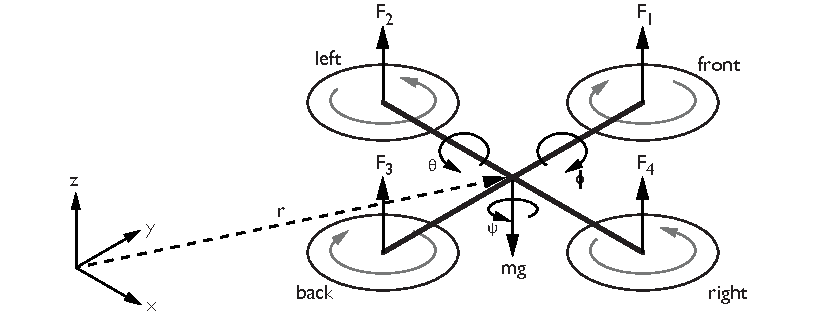
\includegraphics{../fig/quad.pdf}
	\caption[A quadrotor arranged in the cross configuration.]{A quadrotor arranged in the cross configuration. (In the x configuration, the front of the vehicle lies between motors 1 and 2 with the remaining directional labels shifted accordingly.) The position vector of the vehicle's center of mass relative to the inertial reference frame is $r$. Vehicle pitch is $\theta$, roll is $\phi$, and yaw is $\psi$. Motor forces $F_1$, $F_2$, $F_3$, and $F_4$ act upwards in the vehicle's body frame and gravity acts downward in the inertial frame.}
\end{figure}


Advances in Microelectromechanical Systems (MEMS) and light-weight high-powered lithium polymer batteries have contributed to the recent popularity of quadrotors, making them an attractive choice for research applications in flight dynamics and control, as in \cite{hoffmann2007quadrotor, kivrak2006design, mellinger2010control, michael2010grasp}. One problem of particular interest is the development of mathematical models representing system dynamics based on experimentally gathered data through the application of system identification techniques. System identification provides a mechanism to relate this input-output data to the underlying system dynamics, without assuming any a priori knowledge of the system. Traditionally, system identification techniques focused on developing a system model which minimizes prediction error. Identification methods of this form are commonly known as Prediction Error Methods (PEM). PEMs have seen widespread use in both theoretical and real-world applications, but experience difficulties identifying Multi-Input Multi-Output (MIMO) systems \cite{qin2006overview, viberg1995subspace}. 

Subspace Identification Methods (SIM) have recently grown in popularity and offer an alternative approach to the identification problem. SIMs provide an attractive alternative to PEMs because they identify systems directly in their state space form through the application of non-iterative algorithms. These methods have a foundation in linear algebra and overcome the issues found in PEMs when identifying MIMO systems \cite{katayama2005subspace}. While traditional subspace algorithms provide reliable results when identifying systems operating in open-loop, identification of systems operating in closed-loop requires modification of the identification procedure in order to eliminate a bias introduced by the presence of the feedback controller. One such approach, called the Innovation Estimation Method (IEM) pre-estimates the unknown noise sequence before applying a modified subspace identification approach in an attempt to eliminate this bias. It is the goal of this research project to develop a quadrotor model from experimentally gathered closed-loop input-output data using subspace identification with innovation estimation and to evaluate the resulting model's ability to accurately represent the dynamics of the physical quadrotor system.


\section{Related Work}
Developing accurate dynamical models of quadrotors plays an important role in platform development, test, and continuing operational use. Quadrotors are dynamically unstable and are highly nonlinear. Developing system models from first principles is not commonly done due to the complexity of the resulting models and the difficulty of determining the numerous unknown system parameters. Several groups have developed simplified quadrotor models by directly measuring or estimating system parameters \cite{bresciani2008modelling, domingues2009quadrotor, kivrak2006design, pounds2006modelling, schreier2012modeling}, but these models are typically used only to select initial controller gains during control system design and full model simulation results are generally not given. 

Using prediction error techniques has proven to be a viable approach to identifying quadrotor models from input-output data. In \cite{chamberlain2011system}, a system model is identified by applying an AutoRegressive model with eXternal input (ARX) approach using position and attitude data measured by a Cortex 3D camera-based positioning system. In \cite{miller2011open}, NASA's System Identification Programs for Aircraft (SIDPAC) implementation of a least squares PEM is used to individually identify four dynamic modes of a quadcopter (lateral, longitudinal, heave, and yaw) in isolation with output data measured by a Vicon motion capture system. Both cases showed accurate results when comparing predicted system output with measured system response. Model accuracy is boosted in these cases by the use of external camera positioning systems to measure vehicle position and attitude, ensuring the output data used for identification is free from errors introduced by onboard sensor measurements caused by accelerometer drift and vehicle vibrations. When camera positioning systems are not available, it is still possible to identify models using measurements taken by onboard accelerometers and gyroscopes.  A model developed from such onboard data using prediction error in \cite{lee2011attitude} gave acceptable results when simulating pitch and roll dynamics but did not accurately model yaw dynamics.

Subspace identification techniques have also been shown to produce models which accurately describe quadrotor system dynamics. Motor dynamics were identified using Numerical algorithms for Subspace State Space System IDentification (N4SID) in \cite{kis2011sensor} and the resulting model was used to simulate vehicle vertical acceleration. In \cite{batmazdesign}, N4SID was used to identify quadrotor roll dynamics from open-loop data collected by using a test bench setup  which fixed the vehicle pitch and yaw dynamics. 


\section{Motivation and Contributions}
As subspace identification techniques continue to evolve, particularly in emerging areas of research including identification of closed-loop systems, demonstration of empirical results remains important to validate the real world usefulness and applicability of these theories. The motivation for the work presented here is to show empirical results from the development of dynamical models through subspace identification with innovation estimation. Specifically, we analyze whether a six degree of freedom (6DOF) linear time-invariant (LTI) model of a quadrotor operating in closed-loop developed using subspace identification with innovation estimation provides an accurate representation of the true system dynamics.




